\chapter{Laboratorio 3}
\section{Introduzione}
In questa esperienza di laboratorio, è stato analizzato il circuito di amplificazione \textit{common emitter amplifier} con degenerazione di emettitore, nella versione con alimentazione positiva e negativa e nella versione single-ended (\Fig\ref{fig:commonemitter}).
\begin{figure}[h!]
	\centering
	A
	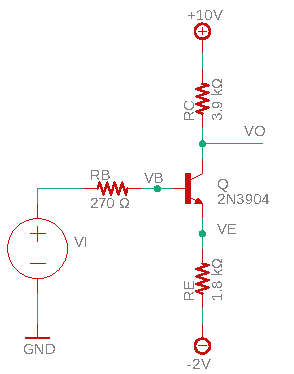
\includegraphics[width=0.4\linewidth]{./OtherFiles/Laboratorio 3/common emitter}
	B
	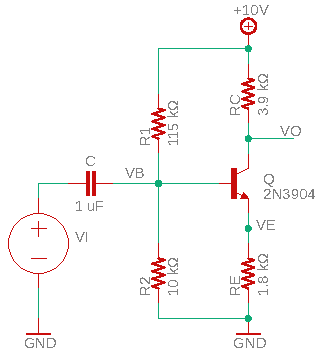
\includegraphics[width=0.4\linewidth]{./OtherFiles/Laboratorio 3/common emitter_se}
	\caption{Schematico del circuito common emitter con degenerazione di emettitore nella versione con alimentazione doppia (A) e singola (B).}
	\label{fig:commonemitter}
\end{figure}

\todo{inserire spiegazione del perchè degenerazione}

\section{Common emitter amplifier: punto di lavoro}
Prima di procedere alla realizzazione dei circuito analizziamone il punto di lavoro.

Consideriamo prima la versione con alimentazione doppia. Supponiamo il transistor in regione attiva diretta, con corrente di base nulla. Allora la tensione al nodo V\sub{B} sarà nulla (corrente nella resistenza R\sub{B} nulla). Allora, ricordando che $V_{BE}=\SI{-0.7}{\volt}$, si deriva che $V_E=\SI{-0.7}{\volt}$. Per cui, la corrente che attraversa la resistenza R\sub{E} è pari a (legge di Ohm) $I_E=\frac{V_E-(\SI{-2}{\volt})}{R_E}$. Dal bilancio di correnti nel transistor, si ricava che $I_C+I_B=I_E$. Dal momento che la corrente di base è considerata nulla, otteniamo che $I_C=I_E$. Ricaviamo poi V\sub{o} tramite legge di Ohm: $I_C=\frac{\SI{10}{\volt}-V_o}{R_C}$, da cui $V_o= \SI{10}{\volt}-R_C*I_C$. Inoltre, ricordiamo che $g_m=\frac{I_C^*}{\phi_T}$, con $I_C^*$ corrente di collettore stazionaria e $\phi_T\simeq\SI{26}{\milli\volt}$. Inoltre, sarà importante verificare che V\sub{BE} sia positiva, in modo da confermare l'ipotesi che il transistor si trova in regione attiva diretta.
\begin{figure}[h!]
	\centering
	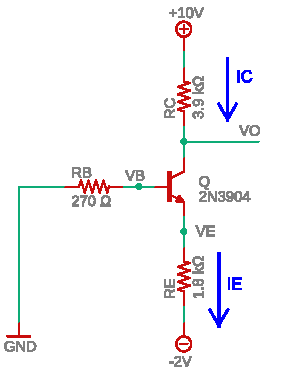
\includegraphics[width=0.4\linewidth]{./OtherFiles/Laboratorio 3/common emitter-punto di lavoro-printout}
	\caption{Analisi del punto di lavoro del circuito common emitter amplifier con alimentazione positiva e negativa.}
	\label{fig:commonemitter_DC}
\end{figure}

Sostituendo i valori dei componenti utilizzati nel circuito otteniamo i seguenti valori, che saranno da confrontare con quelli misurati sul circuito reale:
\begin{table}[h!]
	\centering
	\begin{tabular}{c|c|c|c|c|c}
		\hline
		V\sub{B} [V] & V\sub{E} [V] & V\sub{O} [V] & I\sub{B} [A] & I\sub{E} [mA] & I\sub{C} [mA] \\ \hline
		0 & -0.7 & 7.183  & 0 & 0.7222 & 0.7222 \\ \hline
	\end{tabular}
\end{table}
\todo{inserire tabella nel laboratorio 2}

Procediamo ora con l'analisi del punto di lavoro del circuito \textit{common emitter amplifier}, nella versione con alimentazione singola (\Fig\ref{fig:commonemitter_se_DC}).
\begin{figure}[h!]
	\centering
	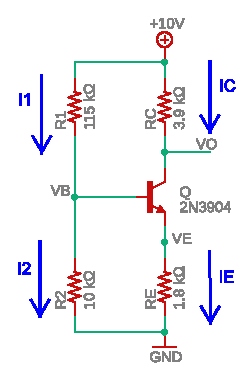
\includegraphics[width=0.4\linewidth]{./OtherFiles/Laboratorio 3/common emitter_se-punto di lavoro-printout}
	\caption{Analisi del punto di lavoro del circuito common emitter amplifier con alimentazione singola.}
	\label{fig:commonemitter_se_DC}
\end{figure}
Supponendo che la corrente di base sia zero (ossia che $\beta_Q\to\infty$), da un bilancio di corrente al nodi V\sub{B} e nel transistor, otteniamo che $I_1=I_2$ e $I_C=I_E$. Si noti che il condensatore è stato considerato come un circuito aperto nell'analisi DC. Infatti, il suo ruolo è quello di disaccoppiare in continua il circuito, in modo che la tensione imposta dal partitore di tensione formato da R\sub{1} e R\sub{2} non sia portata a massa dal generatore V\sub{i}. Infatti, come già discusso in precedenza nell'analisi dell'emitter follower single-ended, le resistenze R\sub{1} e R\sub{2} hanno il compito di alzare la tensione nel nodo V\sub{B}, in modo da mantenere il transistor in zona attiva diretta.

Ricaviamo quindi la tensione V\sub{B} utilizzando la legge di Ohm:
\begin{equation}
	\begin{split}
		I=I_1&=I_2 \\
		\frac{\SI{10}{\volt}-V_B}{R_1}&=\frac{V_B-\SI{0}{\volt}}{R_2} \\
		V_B&=\frac{R_2}{R_1+R_2}*\SI{10}{\volt}
	\end{split}
\end{equation}

La tensione al nodo V\sub{E} è $V_{BE}=V_B-V_E=\SI{0.7}{\volt}$ (transistor in zona attiva diretta), da cui $V_E=V_B-\SI{0.7}{\volt}$. Conoscendo V\sub{E} è ora possibile calcolare la corrente I\sub{E} e I\sub{C} tramite la legge di Ohm: $I_E=I_C=\frac{V_E-\SI{0}{\volt}}{R_E}$. 
Infine, la tensione nel nodo V\sub{O} sarà $V_O=\SI{10}{\volt}-I_C*R*C$. Si dovrà inoltre verificare che la tensione V\sub{CE} sia maggiore di zero.

Sostituendo i valori dei componenti utilizzati nel circuito otteniamo i seguenti valori, che saranno da confrontare con quelli misurati sul circuito reale:
\begin{table}[h!]
	\centering
	\begin{tabular}{c|c|c|c|c|c}
		\hline
		V\sub{B} [mV] & V\sub{E} [mV] & V\sub{O} [V] & I\sub{B} [A] & I\sub{E} [mA] & I\sub{C} [mA]\\ \hline
		800 & 100 & 9.783 & 0 & 0.055 & 0.055\\ \hline
	\end{tabular}
\end{table}

\section{Common emitter amplifier: analisi per piccolo segnale}\label{sec:33}
Analizziamo ora il circuito sotto l'ipotesi di piccolo segnale, utilizzando il modello per piccolo segnale del transistor e spegnendo i generatori di grandezze continue.

Considerando il circuito a emettitore comune con alimentazione doppia si ottiene il circuito in figura \ref{fig:commonemitter_AC}.
\begin{figure}[h!]
	\centering
	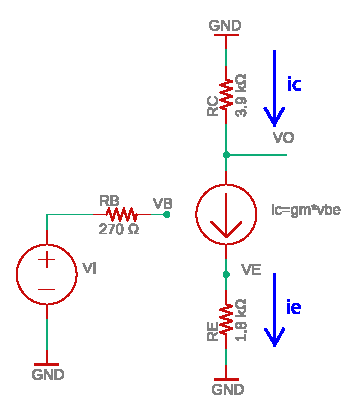
\includegraphics[width=0.4\linewidth]{./OtherFiles/Laboratorio 3/common emitter-piccolo segnale-printout}
	\caption{Analisi per piccolo segnale del circuito common emitter amplifier con alimentazione positiva e negativa.}
	\label{fig:commonemitter_AC}
\end{figure}

Dal momento che nella resistenza R\sub{B} non passa corrente, $v_b=v_i$. Inoltre si possono ricavare le seguenti equazioni (utilizzando legge di Ohm e bilanci di corrente):
\begin{equation}
	\begin{cases}
		i_c=\frac{-v_o}{R_C} \\
		i_c=gm*v_{be}=gm*v_{ie} \\
		i_c=\frac{v_e}{R_E} \\
		i_e=i_c
	\end{cases}
\end{equation}
Risolvendo il sistema, è possibile calcolare la funzione di trasferimento del circuito:
\begin{equation}
	\frac{v_o}{v_i}=-\frac{R_C*g_m}{1+R_E*g_m}\;\underset{g_m*R_E\gg 1}{\simeq}\;-\frac{R_C}{R_E}.
\end{equation}
Il guadagno del circuito è quindi determinato dal rapporto tra la resistenza di collettore e quella di emettitore. Inoltre, la presenza di un segno meno nella funzione di trasferimento indica che il circuito introduce uno sfasamento di \SI{-180}{\degree} tra il segnale in ingresso e quello in uscita (amplificatore invertente). 

L'analisi di piccolo segnale della versione con singola alimentazione è identica a quella presentata precedentemente sotto l'ipotesi che $C\to\infty$, ossia che il condensatore si comporti come un corto circuito per frequenze del segnale sufficientemente alte. Sotto questa ipotesi semplificativa, $v_b=v_i$. Con la risoluzione del medesimo sistema di equazioni si determina che il guadagno è $\frac{v_o}{v_i}\simeq-\frac{R_C}{R_E}.$
\begin{figure}[h!]
	\centering
	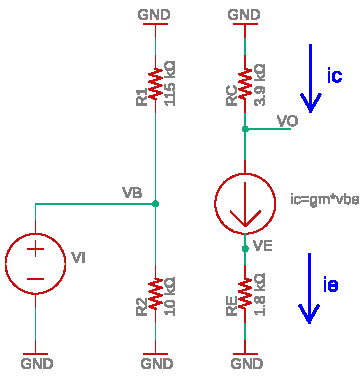
\includegraphics[width=0.4\linewidth]{./OtherFiles/Laboratorio 3/common emitter_se-piccolo segnale-printout}
	\caption{Analisi per piccolo segnale del circuito common emitter amplifier con alimentazione singola.}
	\label{fig:commonemitter_se_AC}
\end{figure}

Sostituendo i valori delle resistenze da utilizzare nei nostri circuiti ci aspettiamo un guadagno di:
\begin{equation}
	\frac{v_o}{v_i}=-\frac{\SI{3.9}{\kilo\ohm}}{\SI{1.8}{\kilo\ohm}}\simeq -2.17.
\end{equation}

\section{Componenti e misure}
I due circuiti sono stati realizzati in laboratorio (\Fig\ref{fig:commonemitter_circuito}).
\begin{figure}[h!]
	\centering
	A)
	
	\includegraphics[width=0.6\linewidth]{./ImageFiles/Laboratorio 3/IMG\_20220524\_110713_2}
	
	B)
	
	\includegraphics[width=0.6\linewidth]{./ImageFiles/Laboratorio 3/IMG\_20220524\_122237\_2}
	\caption{Foto del circuito realizzato in laboratorio nella versione con doppia (A) e singola (B) alimentazione.}
	\label{fig:commonemitter_circuito}
\end{figure}
Per la versione con alimentazione doppia sono stati utilizzati i seguenti componenti:
\begin{itemize}
	\item transistor 2N3904;
	\item una resistenza da \SI{3.9}{\kilo\ohm} per realizzare la resistenza R\sub{C};
	\item una resistenza da \SI{1.8}{\kilo\ohm} per realizzare la resistenza R\sub{E};
	\item una resistenza da \SI{270}{\ohm} per realizzare la resistenza R\sub{B}.
\end{itemize}
Invece per la versione single-ended sono stati utilizzati:
\begin{itemize}
	\item transistor 2N3904;
	\item una resistenza da R\sub{11}=\SI{4.6}{\kilo\ohm} in serie a due resistenze da R\sub{12}=\SI{220}{\kilo\ohm} e R\sub{13}=\SI{220}{\kilo\ohm} connesse in parallelo per realizzare la resistenza R\sub{1};
	\item una resistenza da \SI{12}{\kilo\ohm} per realizzare la resistenza R\sub{2}.
	\item una resistenza da \SI{1.8}{\kilo\ohm} per realizzare la resistenza R\sub{E};
	\item una resistenza da \SI{3.9}{\kilo\ohm} per realizzare la resistenza R\sub{C};
\end{itemize}

Inoltre, sono stati utilizzate i seguenti strumenti:
\begin{itemize}
	\item alimentatore da banco con tensione positiva \SI{10}{\volt}, tensione negativa \SI{-10}{\volt} (utilizzata solo per il circuito con doppia alimentazione)e limite in corrente di \SI{50}{\milli\ampere};
	\item oscilloscopio a due canali;
	\item generatore di forme d'onda;
	\item multimetro da banco.
\end{itemize}

Nelle seguenti tabelle vengono riportate le misure dei componenti usati effettuate tramite il multimetro:

\begin{table}[h!]
	\centering
	\caption{Misure componenti utilizzati per il circuito common emitter amplifier con alimentazione doppia}
	\begin{tabular}{c|c|c}
		\hline
		Componente & Valore nominale & Valore misurato \\ \hline
		R\sub{C} & \SI{3.9}{\kilo\ohm} & \SI{3.962}{\kilo\ohm} \\ \hline
		R\sub{E} & \SI{1.8}{\kilo\ohm} & \SI{1.825}{\kilo\ohm} \\ \hline
		R\sub{B} & \SI{270}{\kilo\ohm} & \SI{274.6}{\ohm} \\ \hline
		Vd\sub{B-E} & $\simeq$ \SI{0.7}{\volt} & \SI{0.700}{\volt} \\ \hline
		Vd\sub{B-C} & $\simeq$ \SI{0.7}{\volt} & \SI{0.679}{\volt} \\ \hline
	\end{tabular}
\end{table}
\begin{table}[h!]
	\centering
	\caption{Misure componenti utilizzati per il circuito common emitter amplifier con alimentazione singola}
	\begin{tabular}{c|c|c}
		\hline
		Componente & Valore nominale & Valore misurato \\ \hline
		R\sub{11} &\SI{220}{\kilo\ohm} & \SI{222.640}{\kilo\ohm} \\ \hline
		R\sub{12} &\SI{220}{\kilo\ohm} & \SI{221.290}{\kilo\ohm} \\ \hline
		R\sub{13} &\SI{4.6}{\kilo\ohm} & \SI{4.639}{\kilo\ohm} \\ \hline
		R\sub{2} &\SI{12}{\kilo\ohm} & \SI{11.883}{\kilo\ohm} \\ \hline
		R\sub{C} & \SI{3.9}{\kilo\ohm} & \SI{3.962}{\kilo\ohm} \\ \hline
		R\sub{E} & \SI{1.8}{\kilo\ohm} & \SI{1.825}{\kilo\ohm} \\ \hline
		Vd\sub{B-E} & $\simeq$ \SI{0.7}{\volt} & \SI{0.700}{\volt} \\ \hline
		Vd\sub{B-C} & $\simeq$ \SI{0.7}{\volt} & \SI{0.679}{\volt} \\ \hline
	\end{tabular}
\end{table}

Una volta realizzato il circuito, sono state misurate le tensioni ai nodi V\sub{B}, V\sub{O} e V\sub{E}, da cui poi è possibile ricavare i valori delle correnti I\sub{C}, I\sub{E} e I\sub{B}. Di seguito sono riportati i risultati per la versione con alimentazione doppia e singola:
\begin{table}[h!]
	\centering
		\caption{Misure dei valori stazionari di tensione e corrente nel circuito common emitter amplifier con alimentazione doppia.}
	\begin{tabular}{c|c|c|c|c|c}
		\hline
		V\sub{B} [mV] & V\sub{E} [V] & V\sub{O} [V] & I\sub{B} [mA] & I\sub{E} [mA] & I\sub{C} [mA]\\ \hline
		-1.056 & -0.655 & 7.080 & -0.0001 & 0.7369 & 0.7370 \\ \hline
	\end{tabular}
\end{table}
\begin{table}[h!]
	\centering
	\caption{Misure dei valori stazionari di tensione e corrente nel circuito common emitter amplifier con alimentazione singola.}
	\begin{tabular}{c|c|c|c|c|c}
		\hline
		V\sub{B} [V] & V\sub{E} [V] & V\sub{O} [V] & I\sub{B} [mA] & I\sub{E} [mA] & I\sub{C} [mA]\\ \hline
		0.920 & 0.304 & 9.334 & 0.0150 & 0.1666 & 0.1681 \\ \hline
	\end{tabular}
\end{table}

Se si confrontano i risultati ottenuti con i valori calcolati nell'analisi teorica del punto stazionario si nota come i valori possono essere considerati corretti con buona approssimazione. \`E curioso osservare che la corrente di base I\sub{B} misurata nel circuito con alimentazione doppia è risultata negativa. Infatti, la corrente di emettitore risulta essere minore della corrente di collettore. Tuttavia, ciò non è ammissibile per costruzione del transistor. Questo risultato però non deve sorprendere in quanto l'errore è dell'ordine di $10^-7$ A. Trattandosi di una corrente molto piccola, gli errori di misura degli strumenti utilizzati per le misure possono aver causato questo risultato.

In seguito è stata misurata la risposta del circuito a un ingresso sinusoidale. 

Per il circuito con alimentazione doppia è stato utilizzato un ingresso sinusoidale di frequenza \SI{1}{\kilo\hertz} e ampiezza picco-picco di \SI{1}{\volt} (\Fig\ref{fig:commonemitter_guadagno}). Calcolando il rapporto tra la resistenza di collettore e quella di emettitore (che determinano il guadagno del circuito) il guadagno atteso è di circa \SI{2.17}. Il guadagno misurato è di circa \SI{2.14}. Si noti inoltre che i segnali sono in contro fase, così come è stato ricavato nell'analisi di piccolo segnale. 

\begin{figure}[h!]
	\centering
	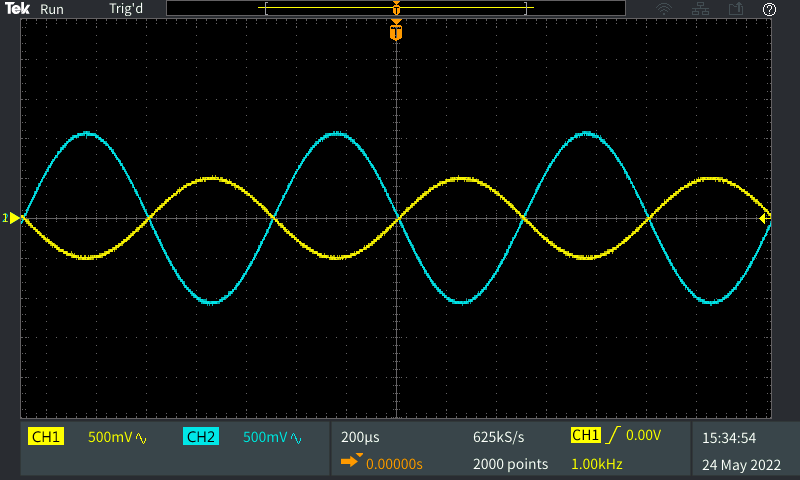
\includegraphics[width=0.7\linewidth]{./ImageFiles/Laboratorio 3/TEK00006}
	\vspace{1cm}
	
	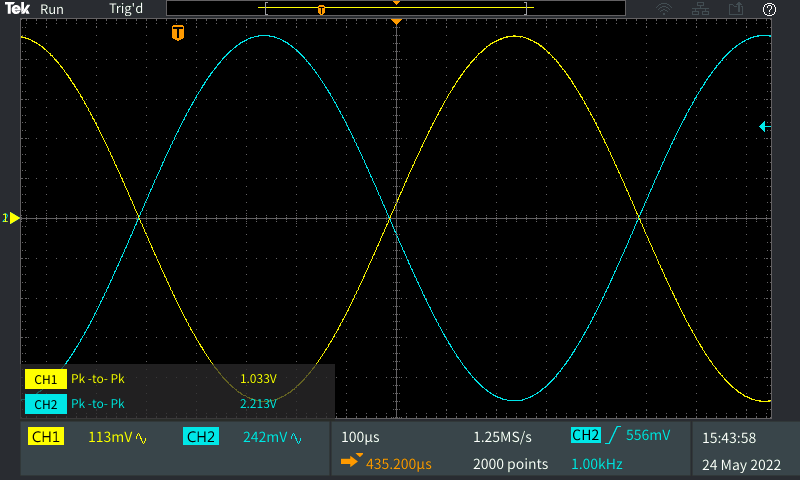
\includegraphics[width=0.7\linewidth]{./ImageFiles/Laboratorio 3/TEK00007}
	\caption{Confronto tra il segnale in ingresso (CH1) e in uscita (CH2) al circuito common emitter amplifier con alimentazione doppia, con onda sinusoidale in ingresso di ampiezza picco-picco di \SI{1}{\volt} e frequenza di \SI{1}{\kilo\hertz}.}
	\label{fig:commonemitter_guadagno}
\end{figure}

Risultati analoghi sono stati misurati sul circuito nella versione single-ended, dove in ingresso è stato applicato un segnale sinusoidale con ampiezza picco-picco di \SI{100}{\milli\volt} e di \SI{1}{\volt}, con frequenza di \SI{1}{\kilo\hertz} (\Fig\ref{fig:commonemitter_se_guadagno}). Il guadagno atteso è il medesimo del circuito precedente. In questo caso il guadagno ottenuto è leggermente inferiore e pari a 1.96, ma comunque prossimo al valore teorico.

\`E importante analizzare il comportamento del circuito nel caso in cui in ingresso è stata fornita un'onda sinusoidale di ampiezza picco-picco di \SI{1}{\volt} (\Fig\ref{fig:commonemitter_se_guadagno}(B)). Infatti, si nota che l'uscita satura alla tensione positiva, in quanto il nodo V\sub{O} si trova ad una tensione di \SI{9.334}{\volt} e, sommandosi la componente di piccolo segnale di ampiezza \SI{500}{\milli\volt}, porterebbe l'uscita ad una tensione superiore all'alimentazione positiva di \SI{10}{\volt}. Ma ciò non è possibile. 

\begin{figure}[h!]
	\centering
	(A)
	
	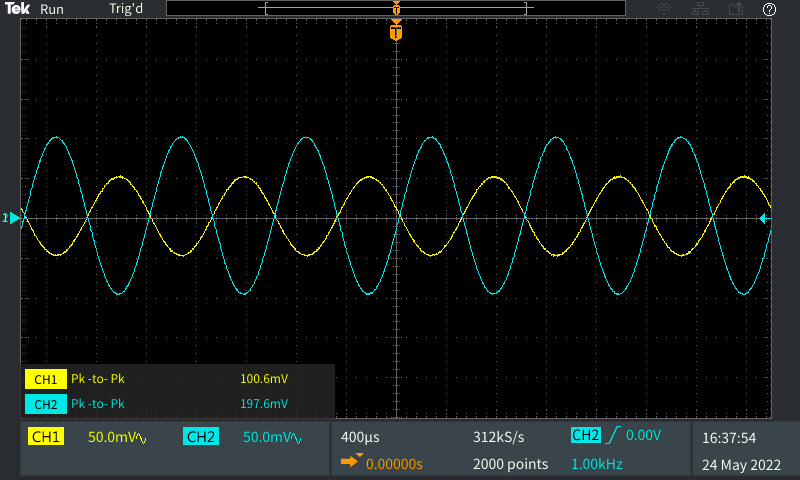
\includegraphics[width=0.7\linewidth]{./ImageFiles/Laboratorio 3/TEK00010}
	\vspace{1cm}
	
	(B)
	
	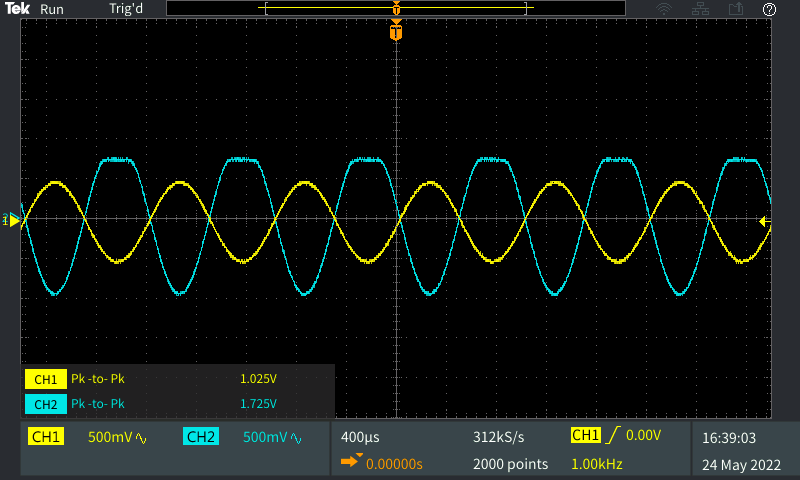
\includegraphics[width=0.7\linewidth]{./ImageFiles/Laboratorio 3/TEK00011}
	\caption{Confronto tra il segnale in ingresso (CH1) e in uscita (CH2) al circuito common emitter amplifier con alimentazione singola, con onda sinusoidale in ingresso di ampiezza picco-picco di \SI{100}{\milli\volt} (A) e \SI{1}{\volt} (B) e frequenza di \SI{1}{\kilo\hertz}.}
	\label{fig:commonemitter_se_guadagno}
\end{figure}

Nella successiva esperienza di laboratorio si analizzerà il comportamento del circuito con un segnale sinusoidale di frequenza minore, dove gli effetti della capacità di disaccoppiamento non sono trascurabili.